\documentclass{article}
\usepackage[UTF8, heading = false, scheme = plain]{ctex}

\usepackage{geometry}
\geometry{b5paper,left=2cm,right=2cm,top=2cm,bottom=2cm}

\usepackage{color}
\usepackage{amsfonts}
\usepackage{amsmath}

\linespread{1.5}

\usepackage[colorlinks,
            linkcolor=red,
            anchorcolor=blue,
            citecolor=green
            ]{hyperref}

\usepackage{listings}
\usepackage{fontspec}
\usepackage{graphicx}
\usepackage{algorithmic}
\newfontfamily\monaco{Monaco}
\definecolor{dkgreen}{rgb}{0,0.6,0}
\definecolor{gray}{rgb}{0.5,0.5,0.5}
\definecolor{mauve}{rgb}{0.58,0,0.82}
\lstset{ %
  basicstyle=\footnotesize\monaco,       % the size of the fonts that are used for the code
  numbers=left,                   % where to put the line-numbers
  numberstyle=\footnotesize\monaco\color{gray},  % the style that is used for the line-numbers
  numbersep=5pt
  stepnumber=1,                   % the step between two line-numbers. If it's 1, each line
                                  % will be numbered
  numbersep=5pt,                  % how far the line-numbers are from the code
  backgroundcolor=\color{white},      % choose the background color. You must add \usepackage{color}
  showspaces=false,               % show spaces adding particular underscores
  showstringspaces=false,         % underline spaces within strings
  showtabs=false,                 % show tabs within strings adding particular underscores
  frame=lines,                   % adds a frame around the code
  rulecolor=\color{black},        % if not set, the frame-color may be changed on line-breaks within not-black text (e.g. commens (green here))
  tabsize=4,                      % sets default tabsize to 2 spaces
  captionpos=t,                   % sets the caption-position to bottom
  breaklines=true,                % sets automatic line breaking
  breakatwhitespace=false,        % sets if automatic breaks should only happen at whitespace
  title=\lstname,                   % show the filename of files included with \lstinputlisting;
                                  % also try caption instead of title
  keywordstyle=\color{blue},          % keyword style
  commentstyle=\color{dkgreen},       % comment style
  stringstyle=\color{mauve},         % string literal style
  escapeinside={\%*}{*)},            % if you want to add LaTeX within your code
  morekeywords={*,...}               % if you want to add more keywords to the set
}

\usepackage{amssymb} 
\usepackage{amsmath}
\usepackage[ruled,vlined]{algorithm2e}

\setlength{\parindent}{2em}

\renewcommand{\G}{\mathbb{G}}
\newcommand{\Z}{\mathbb{Z}}
\newcommand{\Zn}{\mathbb{Z}_n}
\newcommand{\Q}{\mathbb{Q}}

\newcommand{\F}{\mathbb{F}}
\newcommand{\Fq}{\mathbb{F}_q}
\newcommand{\Fp}{\mathbb{F}_p}

\newcommand{\Sbox}{\textsf{Sbox}}
\newcommand{\code}[1]{\lstinline!#1!}

\newcommand{\CKDpriv}{\textsf{CKDpriv}}
\newcommand{\CKDpub}{\textsf{CKDpub}}

%%%%%%%处理下划线:_%%%%%%%%%
\usepackage{underscore}
%%%%%%%处理下划线:_%%%%%%%%%

\setlength{\parindent}{2.1em}

%%%设置页眉和页码格式
\usepackage{fancyhdr}
\newcommand{\makeheadrule}{%
\rule[0.85\baselineskip]{\headwidth}{0.5pt}\vskip-.8\baselineskip}%1.5 0.4->0.5
\makeatletter
\renewcommand{\headrule}{%
{\if@fancyplain\let\headrulewidth\plainheadrulewidth\fi
\makeheadrule}}
\makeatother
\pagestyle{fancy}
\fancyhf{}
\fancyhead[r]{\textit{Crypto In Action}}
\fancyfoot[C]{--{~\thepage~}--}
%%%设置页眉和页码格式结束

\usepackage{color}
\newcommand{\red}{\textcolor{red}}
\newcommand{\blue}{\textcolor{blue}}

\begin{document}

\title{Introducing \textsf{curve25519-dalek}}
\author{longcpp \\ \small{longcpp9@gmail.com}}

\maketitle

基于蒙哥马利曲线Curve25519的$x$坐标系可构建高效安全密钥交换协议\textsf{X25519},
基于与其双向有理等价的Edwards25519曲线上点群可以构建高效率的数字签名算法\textsf{Ed25519}.
为了避免由于因子为8可能导致的基于Edwards25519点群构建的密码协议的安全隐患,
Ristretto技术利用蒙哥马利曲线,扭曲爱德华曲线以及雅各比四次曲线之间的同源性和
商群之间的同构特性,可以从Edwards25519点群中萃取中素数阶点群\textsf{ristretto255}, 
在保留速度等优势的同时,避开了余因子不为1的弊端,为密码协议构建提供坚实的数学结构支撑,
例如Polkadot项目中正是采用了基于\textsf{ristretto255}点群的Schnorr签名算法, \textsf{sr25519}.

Curve25519, Edwards25519以及Ristretto255所依赖的数学理论较为复杂,高效安全实现也有难度.
Rust语言实现的\textsf{curve25519-dalek}库中提供了3种点群的快速实现, 基于该库可实现种类
丰富的密码协议: 
\textsf{x25519-dalek}\footnote{\url{https://github.com/dalek-cryptography/x25519-dalek}}中实现了\textsf{X25519},
\textsf{ed25519-dalek}\footnote{\url{https://github.com/dalek-cryptography/ed25519-dalek}}中实现了\textsf{Ed25519}, 
\textsf{schnorrkel}\footnote{\url{https://github.com/w3f/schnorrkel}}中实现了\textsf{sr25519},
\textsf{zkp}\footnote{\url{https://github.com/dalek-cryptography/zkp}}中实现了Schnorr形式的零知识证明, 
\textsf{bulletproofs}\footnote{\url{https://github.com/dalek-cryptography/bulletproofs}}中实现了零知识证明系统Bulletproof.
本次我们结合数学理论简要介绍\textsf{curve25519-dalek}库提供的接口和功能,

\section{Curve25519与Edwards25519曲线}

先回顾下Curve25519和Edwards25519曲线相关的细节. 蒙哥马利形式的Curve25519曲线是定义在
素数域$\F_p, p = 2^{255}-19$上的, 记为$\mathcal{M}(\F_p)$其曲线方程为
$$
v^2 = u^3 + Au^2 + u, A = 486662\in\F_p,
$$
其中$\#\mathcal{M}(\F_p) = h\cdot\ell, h = 8, 
\ell = 2^{252} + 27742317777372353535851937790883648493$.
单位元为无穷远点$\mathcal{O}_{\mathcal{M}}$, $(0,0)$为2阶点, 
$(1, \sqrt{A+2}), (1, -\sqrt{A+2})$为4阶点, 也即:
$$
\mathcal{M}(\F_p)[4] = \{ \mathcal{O}_{\mathcal{M}}, (0,0), (1, \sqrt{A+2}), (1, -\sqrt{A+2}) \}.
$$
$\mathcal{M}(\F_p)$专用于\textsf{X25519}协议, 而该协议依赖的点群运算仅依赖$u$坐标,
选定的基点为
$$
u(G_{\mathcal{M}}) = \textsf{9}.
$$
$\mathcal{M}(\F_p)$有两个点满足$u$坐标为9,
为了与Edwards25519点群的基点$G_{\mathcal{E}}$相对应, RFC7748中规定:
$$
v(G_{\mathcal{M}}) = 
\textsf{0x5f51e65e475f794b1fe122d388b72eb36dc2b28192839e4dd6163a5d81312c14}.
$$

与$\mathcal{M}(\F_p)$双向有理等价的(Birational Equivalent)扭曲爱德华形式Edwards25519曲线
$\mathcal{E}(\F_p)$的方程为
$$
-x^2 + y^2 = 1 + dx^2y^2, d = -\frac{121665}{121666} \in \F_p, 
$$
并且有$\#\mathcal{E}(\F_p) = \#\mathcal{M}(\F_p)$. 点$(x,y)$的逆元$-(x,y) = (-x,y)$.

\lstinputlisting[language=python, caption=验证Curve25519与Edwards25519, 
label=lst-verify2curve]{curve25519.sage}

\begin{figure}[htbp]
\centering
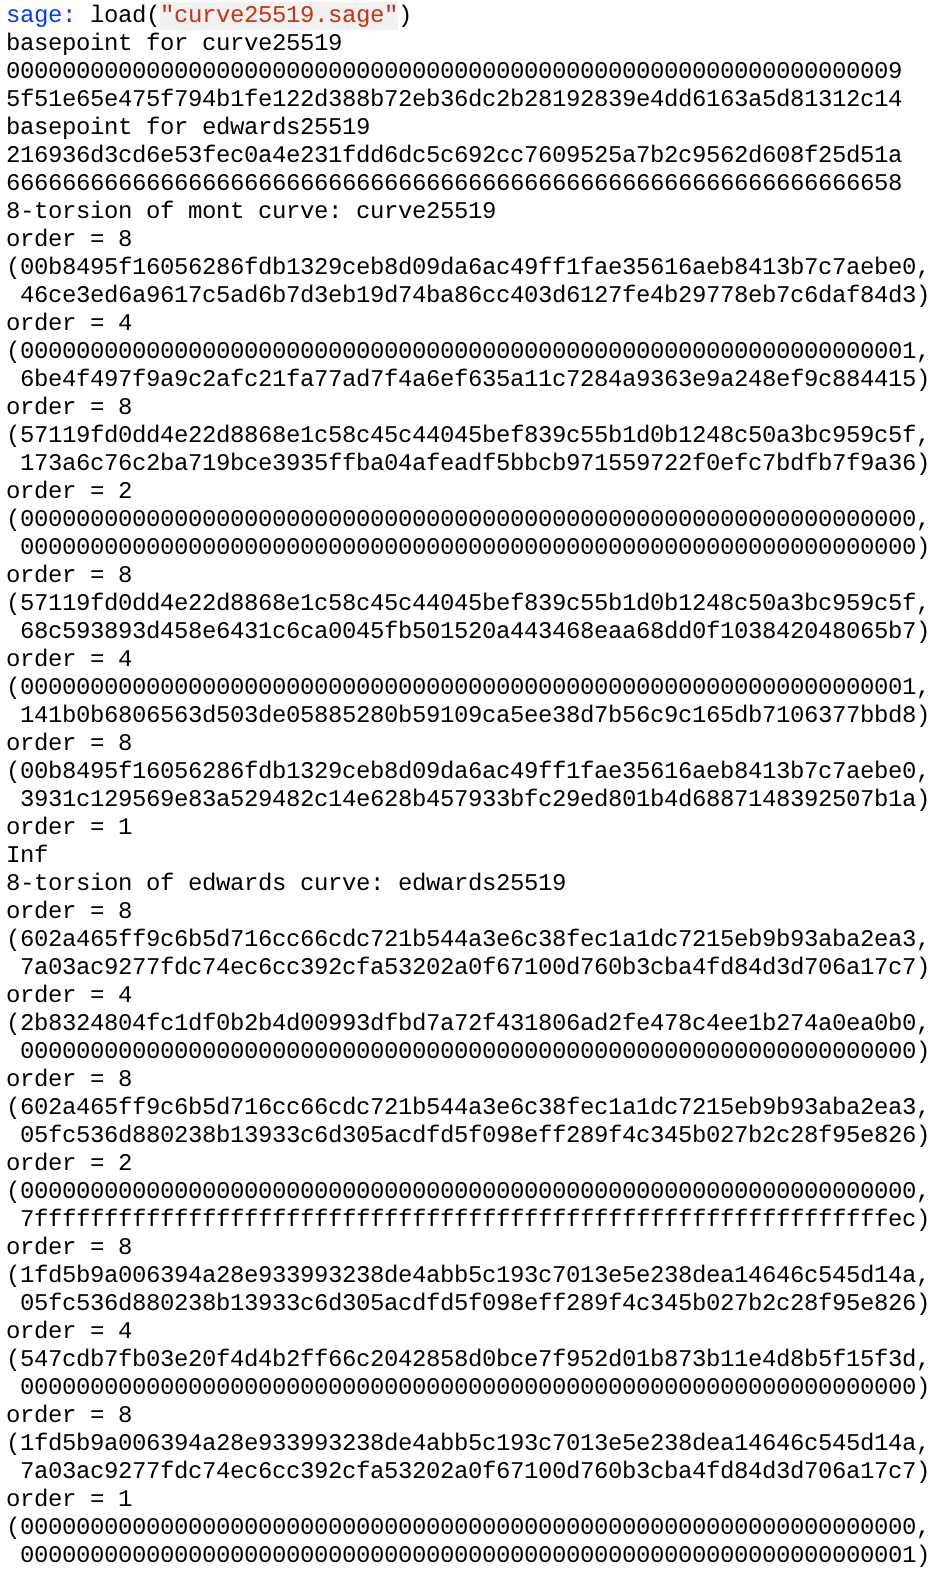
\includegraphics[width=.85\textwidth]{verify2curve.png}
\caption{代码Listing~\ref{lst-verify2curve}~的执行结果}\label{fig-verify2curve}
\end{figure}

$\mathcal{E}(\F_p)$与$\mathcal{M}(\F_p)$之间的双向有理映射为:
$$
(u, v) =  \left( \frac{1+y}{1-y}, \sqrt{-486664}\frac{u}{x} \right), 
(x, y)  =  \left( \sqrt{-486664}\frac{u}{v}, \frac{u-1}{u+1}\right)
$$
其中$(0,1)$为单位元, $(0,-1)$为2阶点, $ (1/\sqrt{-1}, 0), (-1/\sqrt{-1}, 0)$为4阶点, 也即
$$
\mathcal{E}(\F_p)[4] = \{ (0,1), (0,-1), (1/\sqrt{-1}, 0), (-1/\sqrt{-1}, 0) \}.
$$
RFC7748中为$\mathcal{E}(\F_p)$选中的基点$G_{\mathcal{E}}$为:
$$
\begin{array}{rl}
x(G_{\mathcal{E}}) =  & 
\textsf{0x216936d3cd6e53fec0a4e231fdd6dc5c692cc7609525a7b2c9562d608f25d51a}, \\
y(G_{\mathcal{E}}) = & 
\textsf{0x6666666666666666666666666666666666666666666666666666666666666658}.
\end{array}
$$

$\mathcal{E}(\F_p)$与$\mathcal{M}(\F_p)$在代数结构上都同构于$\Z_{h\ell}$,
也即两个点群上的8-torsion $\mathcal{E}(\F_p)[8]$和$\mathcal{M}(\F_p)[8]$均为循环子群,则有
$$
[2]\mathcal{M}(\F_p)[8] =\mathcal{M}(\F_p)[4] ,\ [2]\mathcal{E}(\F_p)[8] = \mathcal{E}(\F_p)[4].
$$
Curve25519和Edwards25519之间的关系可以
通过Listing~\ref{lst-verify2curve}~中展示的Sage代码验证.
代码的执行结果,参见Figure~\ref{fig-verify2curve}, 从中可以看到$G_{\mathcal{M}}$经过函数
\code{mont_to_edwards25519}~变换之后可以得到$G_{\mathcal{E}}$.

\section{\textsf{curve25519-dalek}简介}

\textsf{curve25519-dalek}对外公开的模块有
\code{scalar, montgomery, edwards, ristretto, constants, traits}~等.
\code{scalar}~中实现了$\Z_\ell^*$上的标量运算, \code{montgomery}~中实现了Curve25519上的仅
依赖$u$坐标的点群运算, \code{edwards}~中实现了Edwards25519上的点群运算, 
\code{ristretto}~中通过封装Edwards25519上的点群实现了点群\textsf{ristretto255}上的运算以及编解码功能,
\code{constants}~中则定义了服务于各个模块的常量.
crate内部模块~\code{field}~完成$\F_p$上各种运算, 而具体的运算逻辑则是由~\code{backend}~实现的.
\code{backend}~是可插拔的针对不同平台的实现的$\F_p$内的运算, 例如当存在SIMD指令时,
可以切换到\code{SIMD}后端以加速$\F_p$内的运算. 
内部模块~\code{window}则提供了基于固定窗口(Fixed-Window)和滑动窗口(Sliding-Window)策略的点倍乘运算.

\code{scalar}~中主要定义了~\code{Scalar}~结构体, 用于实现$\Z_\ell^*$上的标量运算.
\code{Scalar}~内部用32字节小端法表示的数组存储$\Z_\ell^*$上的元素. 
为何~\code{scalar}~模块对外公开可用,而~\code{field}~模块仅对crate内部公开?
这是因为在各种密码协议中, 私钥为$\Z_\ell^*$中的元素, 
而公钥为点群中的点, $\F_p$相关逻辑隐藏在了点运算内部, 因此库的用户通常无需关心$\F_p$相关接口.

点群的通用接口定义在~\code{traits}~模块中,其中抽象了$\mathcal{M}(\F_p)$, $\mathcal{E}(\F_p)$
以及\textsf{ristretto255}这3个点群可以支持的方法:
\begin{enumerate}
\item 获得群上的单位元~\code{Identity}, 判断是否为单位元~\code{IsIdentity}
\item 判断一个点是否在曲线上的函数~\code{ValidityCheck}.
\item 没有预计算的常量时间多标量乘法运算~\code{MultiscalarMul}, 
\item 没有预计算且不保证常量时间的多标量乘法运算~\code{VartimeMultiscalarMul}, 
\item 有预计算且不保证常量时间的多标量乘法运算~\code{VartimePrecomputedMultiscalarMul}:
	\begin{enumerate}
	\item 仅有固定点时多标量乘法:~\code{vartime_multiscalar_mul}
	\item 计算在仅有固定点时的多标量乘法~\code{vartime_multiscalar_mul}
	\item 有动态点且不一定是合法时的多标量乘法~\code{optional_mixed_multiscalar_mul}
	\end{enumerate}
\end{enumerate}
\code{traits}~模块中点群方法的实例化是在~\code{montgomery, edwards, ristretto}~模块中完成的.

\code{montgomery}~中定义了$\mathcal{M}(\F_p)$上的点群~\code{MontgomeryPoint}~和相应运算,
如前所述该点群中的运算仅依赖$u$坐标系, 无穷远点的$\mathcal{O}_{\mathcal{M}}$对应的$u$坐标为0.
\code{MontgomeryPoint}~结构体内部为小端法表示的32字节数组, 这是因为$u\in\F_p, p < 2^{256}$.
因此借助~\code{as_bytes}~或者~\code{to_bytes}~可以查看~\code{MontgomeryPoint}~的值.
关于点的倍乘方面, ~\code{MontgomeryPoint}~仅用来
实现X25519协议, 而该协议仅需要单点的倍乘运算,
因此~\code{montgomery}不支持~\code{traits}~中多标量乘法运算.

值得注意的是, 通过函数~\code{to_edwards}~可以将~\code{MontgomeryPoint}~转换
成~\code{edwards}~模块中定义的~\code{EdwardsPoint}, 
不是所有的$u\in\F_p$都位于曲线Curve25519上
(可能位于Curve25519的二次扭曲线上\footnote{longcpp. 深入理解X25519. 
\url{https://github.com/longcpp/CryptoInAction/blob/master/intro-ed25519/190902-intro-x25519.pdf}})
也即不是所有的~\code{MontgomeryPoint}~都可以转换成~\code{EdwardsPoint}, 
因此~\code{to_edwards}~的返回值为~\code{Option<EdwardsPoint>}.
另外一个~\code{MontgomeryPoint}~可以映射成2个~\code{EdwardsPoint},
可以通过输入参数指定具体要映射到哪个点. 
~\code{to_edwards}~具体实现可以参考Listing~\ref{lst-mont-to-edwards}.
从~\code{MontgomeryPoint}~转换到~\code{EdwardsPoint}的具体运算是按照
从$\mathcal{M}(\F_p)$到$\mathcal{E}(\F_p)$的映射$y = (u-1)/(u+1)$进行计算的.
这就要求$u\neq -1$, 又注意到$u = -1$时, 根据$\mathcal{M}(\F_p)$方程有:
$v^2 = -1 + 486662 - 1 = 486660$, 然而48000是$\F_p$上的二次非剩余,
也即$u = -1$时对应的点位于Curve25519的二次扭曲线上, 此时~\code{to_edwards}~直接返回~\code{None}.
\code{to_edwards}~是借助~\code{edwards}~模块中定义的另一个结构体
\code{CompressedEdwardsY}来完成的到~\code{EdwardsPoint}~的转换.

\begin{lstlisting}[caption=\code{MontgomeryPoint}的~\code{to_edwards}~实现, label=lst-mont-to-edwards]
pub fn to_edwards(&self, sign: u8) -> Option<EdwardsPoint> {
    let u = FieldElement::from_bytes(&self.0);
    
    if u == FieldElement::minus_one() { return None; } // u = -1
    
    let one = FieldElement::one();
    
    let y = &(&u - &one) * &(&u + &one).invert(); // u = (u-1) / (u+1)

    let mut y_bytes = y.to_bytes();
    y_bytes[31] ^= sign << 7; // 最高位保存输入参数sign

    CompressedEdwardsY(y_bytes).decompress()
}
\end{lstlisting}

\code{edwards}模块中的~\code{CompressedEdwardsY}~结构体是~\code{EdwardsPoint}~的压缩表示形式:
仅用$y\in\F_p$以及$x$坐标正负来表示一个点. 由于$p < 2^{255}$, 所以用32字节的数字来存储$y$的值,
并且最高位可以用来存储$x$的正负号,因此~\code{CompressedEdwardsY}~仅需要32个字节来存储.
\code{EdwardsPoint}~可以通过~\code{compress}~方法转换为~\code{CompressedEdwardsY},
参见Listing~\ref{lst-edwards-compressY}. 为了理解~Listing~\ref{lst-edwards-compressY},
需要解释下~\code{EdwardsPoint}~的定义.为了提高运算效率,  \textsf{curve25519-dalek}中为
\code{EdwardsPoint}~选取的坐标系为扩展的扭曲爱德华坐标系的坐标表示, 仿射坐标系下的点$(x,y)$
对应该坐标系下的点$(X:Y:Z:T)$, 其中$x = X/Z, y = Y/Z, xy = T/Z$.
可以注意到Listing~\ref{lst-mont-to-edwards}~和Listing~\ref{lst-edwards-compressY}
对符号位的处理是一致的. \code{CompressedEdwardsY}通过~\code{decompress}~方法转换为
\code{EdwardsPoint}~, 此处不再展示相应实现.
\code{EdwardsPoint}~可以通过~\code{to_montgomery}~方法转换成~\code{MontgomeryPoint}.

\begin{lstlisting}[caption=\code{EdwardsPoint}的~\code{compress}~实现, label=lst-edwards-compressY]
/// Compress this point to `CompressedEdwardsY` format.
pub fn compress(&self) -> CompressedEdwardsY {
    let recip = self.Z.invert(); // Z^-1
    let x = &self.X * &recip; // x = X/Z
    let y = &self.Y * &recip; // y = Y/Z
    let mut s: [u8; 32]
    
    s = y.to_bytes();
    s[31] ^= x.is_negative().unwrap_u8() << 7; // 在最高位保存x的符号
    CompressedEdwardsY(s)
}
\end{lstlisting}

当基于余因子不为1的点群构建密码协议时, 常会在不经意间引入安全隐患.\footnote{
longcpp. Edwards25519余因子与双花交易.
\url{https://github.com/longcpp/CryptoInAction/blob/master/intro-ed25519/200212-edwards25519-cofactor.pdf}}
方便起见, \code{edwards}~模块提供了工具函数~\code{is_small_order}~来判断点是否属于$\mathcal{E}(\F_p) [8]$,
也提供了函数~\code{is_torsion_free}~来判断点是否属于$ \mathcal{E}(\F_p)[\ell]$, 也即``torsion-free''.
为了理解``torsion-free''的概念, 考虑
$$\mathcal{E}(\F_p) \cong \mathcal{E}(\F_p) [8] \times \mathcal{E}(\F_p)[\ell],$$
并且$H \in  \mathcal{E}(\F_p) [8],\ G\in \mathcal{E}(\F_p)[\ell]$为子群的生成元,
则所有的$P \in \mathcal{E}(\F_p)$都可以表示为 $P = xG + yH, x\in \Z_\ell, y\in\Z_8$.
当$P$为``torsion-free''时, 意味着$P= xG+ yH$中$y = 0$. 
注意到$\textsf{gcd}(8,\ell) = 1$, 则``torsion-free''也等价于$\ell P = (0,1)$(注意$(0,1)$为单位元).

\code{ristretto}~模块利用Ristretto技术从基于$\mathcal{E}(\F_p)$萃取出素数阶$\ell$的点群\textsf{ristretto255}.
Ristretto技术的数学原理参见\footnote{longcpp. Ristretto: 萃取素数阶点群.
\url{https://github.com/longcpp/CryptoInAction/blob/master/intro-ed25519/200324-intro-ristretto.pdf}}
以及~\textsf{curve25519-dalek}~的文档\footnote{
The Ristretto Group\url{The Ristretto Group}}.
依赖蒙哥马利曲线, 扭曲爱德华曲线以及雅各比四次曲线之间的同源关系以及某些商群之间的同构关系
的Ristretto技术原理比较繁杂, 但是可以简单的概述为点扭曲爱德华曲线上的点$P\in [2]\mathcal{E}(\F_p)$,
经过扭转(Torquing), 曲线之间的同源关系(Isogeny)以及商群(Quotient Group)之间的同构(Isomorphism),
最终被编码为雅各比四次曲线(Jacobi Quartic Curve)点群$\mathcal{J}(\F_p)$
与其2-torsion$\mathcal{J}(\F_p)[2]$的
商群$\mathcal{J}(\F_p)/\mathcal{J}(\F_p)[2]$的规范表示(Canonical Representation).
理解$\textsf{ristretto255}$并不需要理解前面这句话.
相比繁杂的Ristretto技术原理, 基于$\mathcal{E}(\F_p)$实现点群\textsf{ristretto255}的逻辑相对清晰.
值得指出的是,虽然根据Ristretto技术原理, $\textsf{ristretto255}$经过快速转换之后可以参与
蒙哥马利阶梯算法, 但是~\textsf{curve25519-dalek}~中没有实现这一过程.
另外值得注意的是, $\textsf{ristretto255}$点群仅处理了$P\in [2]\mathcal{E}(\F_p)$的点,
这涵盖了$\mathcal{E}(\F_p)[4]\times\mathcal{E}(\F_p)[\ell]$的点.

正如Mike Hamberg在Decaf论文中提到的(Ristretto技术是通过扩展Decaf技术而得到的),
基于一个点群实现萃取素数阶点群,只需要重新定义点的编解码以及点相等的判断逻辑.
具体的点群运算,可以将萃取出来的点群上的点转化为适当的点格式基于已有的实现完成运算.
\textsf{curve25519-dalek}~中的实现正是如此. \code{ristretto}~模块定义了两种点格式
~\code{RistrettoPoint}~以及~\code{CompressedRistretto}, 从两种结构体的定义中可以
看到具体的~\textsf{curve25519-dalek}~中$\textsf{ristretto255}$的实现策略,
参见Listing~\ref{lst-ristretto-point}. 由于
$$
\mathcal{E}(\F_p)[4] = \{ (0,1), (0,-1), (1/\sqrt{-1}, 0), (-1/\sqrt{-1}, 0) \},
$$
所以对于任意的~\code{EdwardsPoint}~$P=(x,y)\in\mathcal{E}(\F_p)[\ell]$, 
根据Ristretto编码, 点$P$关于$\mathcal{E}(\F_p)[4]$的陪集中的四个点
$$
P + \mathcal{E}(\F_p)[4] = \{ (x,y), (-x,-y), (y/\sqrt{-1}, -\sqrt{-1}x), (-y/\sqrt{-1}, \sqrt{-1}x) \}.
$$
在Ristretto编码下会得到相同的编码值,也即相同的~\code{CompressedRistretto}.

\begin{lstlisting}[caption=\code{RistrettoPoint}~和~\code{CompressedRistretto}~定义, label=lst-ristretto-point]
/// A `RistrettoPoint` represents a point in the Ristretto group for
/// Curve25519.  Ristretto, a variant of Decaf, constructs a
/// prime-order group as a quotient group of a subgroup of (the
/// Edwards form of) Curve25519.
///
/// Internally, a `RistrettoPoint` is implemented as a wrapper type
/// around `EdwardsPoint`, with custom equality, compression, and
/// decompression routines to account for the quotient.  This means that
/// operations on `RistrettoPoint`s are exactly as fast as operations on
/// `EdwardsPoint`s.
///
#[derive(Copy, Clone)]
pub struct RistrettoPoint(pub(crate) EdwardsPoint);


/// A Ristretto point, in compressed wire format.
///
/// The Ristretto encoding is canonical, so two points are equal if and
/// only if their encodings are equal.
#[derive(Copy, Clone, Eq, PartialEq)]
pub struct CompressedRistretto(pub [u8; 32]);
\end{lstlisting}

Listing~\ref{lst-ristretto-point}~中可以看到~\code{RistrettoPoint}~结构体的定义
其实是~\code{EdwardsPoint}~的简单封装. 这意味着~\code{RistrettoPoint}~的点群运算
实际上是通过~\code{EdwardsPoint}~的点群运算完成的.
将~\code{RistrettoPoint}~转换为~\code{CompressedRistretto}~也就完成了
点群\textsf{ristretto255}中点的编码, 
相应逻辑实现在~\code{RistrettoPoint}~的~\code{compress}~方法中.
\code{compress}~方法在扩展的扭曲爱德华坐标系下,严格按照Ristretto编码方式完成.
解码方式则实现在~\code{CompressedRistretto}~的~\code{decompress}~方法中.
2个~\code{RistrettoPoint}~相等的判断在~\code{RistrettoPoint}~的~\code{ct_eq}~方法中实现,
参见Listing~\ref{lst-ristretto-eq}, 相关的逻辑解释请参考\footnote{longcpp. Ristretto: 萃取素数阶点群.
\url{https://github.com/longcpp/CryptoInAction/blob/master/intro-ed25519/200324-intro-ristretto.pdf}}.

\begin{lstlisting}[caption=\code{RistrettoPoint}~的~\code{ct_eq}~方法, label=lst-ristretto-eq]
impl ConstantTimeEq for RistrettoPoint {
    /// Test equality between two `RistrettoPoint`s.
    ///
    /// # Returns
    ///
    /// * `Choice(1)` if the two `RistrettoPoint`s are equal;
    /// * `Choice(0)` otherwise.
    fn ct_eq(&self, other: &RistrettoPoint) -> Choice {
        let X1Y2 = &self.0.X * &other.0.Y;
        let Y1X2 = &self.0.Y * &other.0.X;
        let X1X2 = &self.0.X * &other.0.X;
        let Y1Y2 = &self.0.Y * &other.0.Y;

        X1Y2.ct_eq(&Y1X2) | X1X2.ct_eq(&Y1Y2)
    }
}
\end{lstlisting}

值得提及的是, \code{ristretto}~模块内部还提供了Elligator映射, 该映射本质上实现了哈希到点群的逻辑.
Elligator映射不是外部接口,但可经由外部接口调用.
\code{RistrettoPoint::random()}~用来从随机数发生器生成\textsf{ristretto255}中的随机点,
\code{RistrettoPoint::from_hash()}和~\code{RistrettoPoint::hash_from_bytes()}~完成哈希到点群的逻辑.
至此~\code{curve25519-dalek}~中最为关键的三种点群已经介绍完,
他们之间的逻辑关系参见Figure~\ref{fig-curve25519dalek}.

\begin{figure}[htbp]
\centering
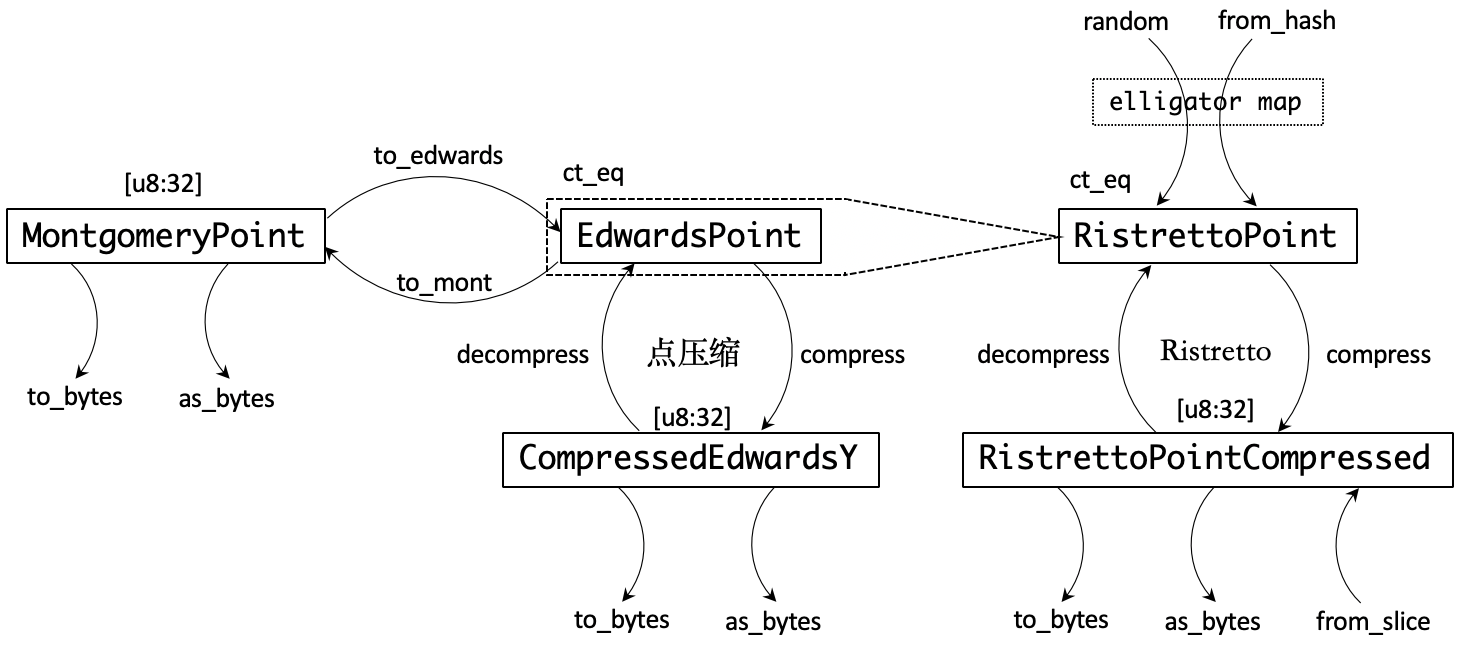
\includegraphics[width=\textwidth]{curve25519-dalek.png}
\caption{\code{curve25519-dalek}中点群间的关系}\label{fig-curve25519dalek}
\end{figure}

code{constants}~模块中定义了3个点群中的常量, 如$\ell$用~\code{BASEPOINT_ORDER}~表示,
\code{X25519_BASEPOINT}~是X25519协议选用的基点$G_{\mathcal{M}}$,
$\mathcal{E}(\F_p)$大素数阶子群$\mathcal{E}(\F_p)[\ell]$的基点$G_{\mathcal{E}}$及其压缩表示
\code{ED25519_BASEPOINT_POINT}, \code{ED25519_BASEPOINT_COMPRESSED}.
\code{EdwardsPoint}~形式表示的8阶循环子群$\mathcal{E}(\F_p)[8]$
由8个元素的数组~\code{EIGHT_TORSION}~表示. 
值得提及的是, \code{EIGHT_TORSION}~下标为0,2,4,6的
4个~\code{EdwardsPoint}~记为$\mathcal{E}(\F_p)[4]$.
由此可以理解~\code{RistrettoPoint}~的~\code{coset4}~方法返回的陪集, 
参见Listing~\ref{lst-ristretto-coset4}.
点群\textsf{ristretto255}的基点定义为~\code{RISTRETTO_BASEPOINT_POINT},
其压缩表示形式为~\code{RISTRETTO_BASEPOINT_COMPRESSED}.
接下来介绍基于\textsf{curve25519-dalek}实现的\textsf{X25519},
\textsf{Ed25519}以及\textsf{sr25519}协议, 这3个协议分别用到了
\code{MontgomeryPoint}, \code{EdwardsPoint}~以及~\code{RistrettoPoint}.

\begin{lstlisting}[caption=\code{RistrettoPoint}~的~\code{coset4}~方法, label=lst-ristretto-coset4]
/// Return the coset self + E[4], for debugging.
fn coset4(&self) -> [EdwardsPoint; 4] {
    [  self.0
    , &self.0 + &constants::EIGHT_TORSION[2]
    , &self.0 + &constants::EIGHT_TORSION[4]
    , &self.0 + &constants::EIGHT_TORSION[6]
    ]
}
\end{lstlisting}


\end{document}